\chapter{Methodology}
\label{Chapeter3}
\lhead{Chapter 3. \emph{Methodology}}  
This chapter outlines the methodology followed in this work to perform the computational simulations of calcium silicate hydrates (C-S-H). All the calculateions were carried out using Density Functional Tight Binding (DFTB+)---primarily in the initial stages---and subsequently with the Vienna Ab-initio Simulation Package (VASP).

We begin by describing the initial C-S-H structure, followed by a preliminary relaxation using DFTB+. Thereafter, we present the workflow adopted in VASP, detailing the main input and output files necessary for the simulations. Finally, we discuss the generation of the  machine learning force field (MLFF), covering the training, refinement and testing phases. 

\section{Initial CSH Structure}
The investigations performed in this work are based in the C-S-H structure proposed by Pellenq \emph{et al.}\supercite{Pellenq2009}. 
This molecular model was constructed 


\begin{figure}[h]
    \centering
    \includegraphics[width=1\textwidth]{POSCAR-extra-colours.png}
    \caption{Molecular model of C-S-H proposed by Ref.\supercite{Pellenq2009}. Lavender and white spheres are oxygen and hydrogen from  water molecules respectively; light blue and brown spheres are inter and intra-layer calcium ions, respectively; electric blue and red spheres are silicon and oxigen atoms from silica tetrahedra, respectively. 
    }
    \label{fig:csh_structure}
\end{figure}


\section{VASP Workflow}
\begin{figure}[h]
    \centering
    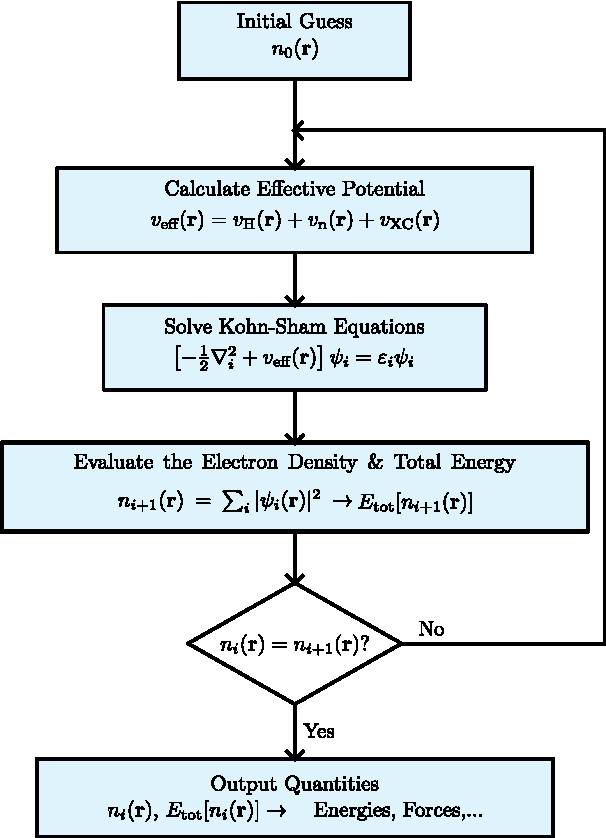
\includegraphics[width=0.6\textwidth]{vasp-workflow.pdf}
    \caption{
        Self-consistent field (SFC) cycle in VASP for DFT calculations adapted from Ref.\supercite{sholl2023density}. The entire cycle starts with an initial guess of the electronic density $n_0(\mathbf{r})$, which then is used to calculate the effective potential $v_{\text{eff}}(\mathbf{r})$. Then, the resulting potential is used to solve the Kohn-Sham equations, from which single-electron wavefunctions $\psi_i(\mathbf{r})$ are obtained. Consequently, the new electronic density $n_{i+1}(\mathbf{r})$ is calculated. Should the old and new densities be close enough---up to a predefined threshold---the cycle stops, and the final electronic density is used to calculate the energies, forces and stress tensor of the system. Otherwise, the cycle repeats itself until convergence is achieved. 
    }
    \label{fig:vasp_workflow}
\end{figure}

\section{VASP Input \& Output Files}
One more section
\subsection{Input Files}

\begin{figure}[h]
\resizebox{\textwidth}{!}{
\begin{tabular}{>{\columncolor{blue!10}}c>{\columncolor{blue!10}}c>{\columncolor{blue!10}}c
>{\columncolor{blue!10}}l>{\columncolor{blue!10}}l>{\columncolor{blue!10}}l>{\columncolor{blue!10}}l
>{\columncolor{blue!10}}l>{\columncolor{blue!10}}l>{\columncolor{blue!10}}l>{\columncolor{blue!10}}l
>{\columncolor{blue!10}}l>{\columncolor{blue!10}}l>{\columncolor{blue!10}}l>{\columncolor{blue!10}}l
>{\columncolor{blue!10}}l>{\columncolor{blue!10}}l>{\columncolor{blue!10}}l>{\columncolor{blue!10}}l
>{\columncolor{blue!10}}l>{\columncolor{blue!10}}l>{\columncolor{blue!10}}l>{\columncolor{blue!10}}l
>{\columncolor{blue!10}}l>{\columncolor{blue!10}}l}
\hline
\multicolumn{3}{l}{\cellcolor{blue!10} \textbf{Ca Si O H}} & & & & & & & & & & & & & & & & & & & & & & \\
\multicolumn{3}{l}{\cellcolor{blue!10}1.0} & & & & & & & & & & & & & & & & & & & & & & \\
13.18335946 & 0.18445997 & 0.00755401 & & & & & & & & & & & & & & & & & & & & & & \\
-16.45244030 & 24.21622147 & -0.00875423 & & & & & & & & & & & & & & & & & & & & & & \\
1.20664987 & -0.82375620 & 23.18729854 & & & & & & & & & & & & & & & & & & & & & & \\
\multicolumn{3}{l}{\cellcolor{blue!10} \textbf{Ca Si O H}} & & & & & & & & & & & & & & & & & & & & & & \\
\multicolumn{3}{l}{\cellcolor{blue!10}99 60 323 208} & & & & & & & & & & & & & & & & & & & & & & \\
\multicolumn{3}{l}{\cellcolor{blue!10}Direct} & & & & & & & & & & & & & & & & & & & & & & \\
0.38821570 & 0.10613519 & 0.29312228 & & & & & & & & & & & & & & & & & & & & & & \\
0.37259751 & 0.56538816 & 0.26881558 & & & & & & & & & & & & & & & & & & & & & & \\
0.37469040 & 0.31600944 & 0.23882914 & & & & & & & & & & & & & & & & & & & & & & \\
0.35542617 & 0.78384113 & 0.38748504 & & & & & & & & & & & & & & & & & & & & & & \\
0.91347068 & 0.11233954 & 0.31634176 & & & & & & & & & & & & & & & & & & & & & & \\
0.90355777 & 0.57838562 & 0.23567872 & & & & & & & & & & & & & & & & & & & & & & \\
0.87836092 & 0.32109531 & 0.25338100 & & & & & & & & & & & & & & & & & & & & & & \\
0.84529168 & 0.81264469 & 0.29236748 & & & & & & & & & & & & & & & & & & & & & & \\
0.11769176 & 0.02588977 & 0.65372010 & & & & & & & & & & & & & & & & & & & & & & \\
\hline
\end{tabular}
}
\caption{Unit cell structure in fractional coordinates for the \ce{C-S-H} (Calcium-Silicate-Hydrate) system. The lattice vectors, atomic species (99 Ca, 60 Si, 323 O, 208 H), and the first 9 atomic positions are shown. All coordinates are expressed in direct (fractional) form.}
\label{fig:csh_poscar}

\end{figure}

\subsection{Output Files}

\section{Strucure Optimisation and Relaxation}
\subsection{Initial Relaxation with DFTB+}
\subsection{Full Structure Relaxation with VASP}
\section{Machine Learning Force Field Generation}
\subsection{MLFF Training}
\subsection{MLFF Refinement}
\subsection{MLFF Testing}

One last section 

